\subsubsection{NATaS}
Pour paralléliser le SpMV, nous utilisons du parallélisme de boucle.
%
Notre ordonnanceur NUMA, NATaS, prend en charge ce type de parallélisme.
%
En plus d'optimiser le placement des pages, il répartira la charge de travail en prenant en compte la localité mémoire.
%
Sur le cas à 8 variables primaires, nous obtenons les mêmes performances qu'en mémoire distribuée (Fig.~\ref{fig:res_spmv_nas}).
%
Pour 3 variables primaires, nous obtenons 95~\% des performances de la version en mémoire distribuée.
%
Par contre, nous n'obtenons que 70~\% avec 1 variable primaire.

%   (-_-)   %
\begin{figure}[t!]
  \centering
  \includegraphics[width=0.7\textwidth]{res_spmv_nas}
  \caption{Accélération du produit matrice vecteur creux sur Rostand en mémoire partagée avec NATaS.}
  \label{fig:res_spmv_nas}
\end{figure}


Malheureusement, sur la machine Manumanu, malgré un placement optimal des pages mémoires, NATaS ne fait pas aussi bien que MPI (Fig.~\ref{fig:res_spmv_nas_manumanu}).
%
Cela provient en grande partie de l'architecture logicielle de NATaS.
%
Nous effectuons trop d'accès à un ensemble de variables partagées par tous les threads.
%
Pour améliorer considérablement les performances, il faudrait construire un ordonnanceur utilisant moins de variables partagées.
%
Mais ce type d'ordonnanceur est dur à écrire, nos machines de calculs étant essentiellement composées de 2 bancs NUMA, il n'y a aucune volonté de notre côté pour écrire cet ordonnanceur.
%
L'utilisation de 2 bancs NUMA nous donne une accélération de 10, tout comme la version en mémoire distribuée.
%
Au delà de 2 bancs NUMA, les performances sont légèrement meilleures que la version OpenMP, atteignant une accélération de 40.

%   (-_-)   %
\begin{figure}[t!]
  \centering
  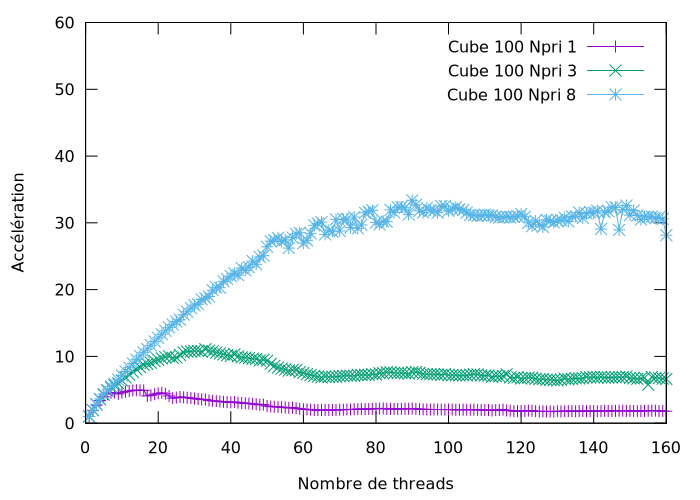
\includegraphics[width=0.7\textwidth]{res_spmv_nas_manu}
  \caption{Accélération du produit matrice vecteur creux sur Manumanu en mémoire partagée avec NATaS.}
  \label{fig:res_spmv_nas_manumanu}
\end{figure}
